\chapter{Fermi-LAT Observations of Extended Gamma-Ray Emission in the Direction of SNR G150.3+4.5.}
\label{chap:G150}


%%%%%%%%%%%%%%%%%%%%%%%%%%%%%%%%%%%%%%%%%%%%%%%%%%%%%%%%%%%%%%%%
%
%         Introduction 
%
%%%%%%%%%%%%%%%%%%%%%%%%%%%%%%%%%%%%%%%%%%%%%%%%%%%%%%%%%%%%%%%%

\section{Introduction}\label{G150:intro}
SNRs have long been thought to be the most-likely accelerators of \crs{} up to the knee of the CR energy spectrum, with diffusive shock acceleration being the primary mechanism accelerating the charged particles to \gam{} emitting energies (see \cite{Reynolds08} for a review of  SNRs from X-rays to \gam{}s ). \Fermi{}-LAT was instrumental \jamie{pun!} in demonstrating that CR protons can indeed be accelerated by SNR shock fronts (through detection of the characteristic "pion bump" feature), and are capable of generating the observed \gam{} emission in SNRs \citep{W44pion, Jogler16}. In addition, observations of SNRs with the LAT have proven to be vital in uncovering a large swath of the \gam{} SNR population; both evolved SNRs interacting with dense surrounding material, as well as dynamically young remnants useful for probing acceleration directly at the shock \citep{snrCat}. 

The  recently updated Pass 8 LAT event reconstruction provides a significantly improved angular resolution,  acceptance, and background event rejection \citep[and Chapter \ref{FGST:analysis}]{atwood13b,atwood13}, all of which lead to an increase in the effective energy range and sensitivity of the LAT. Leveraging the increased sensitivity afforded by Pass 8 data, \cite{2FHL} performed an all-sky analysis from 50 GeV to 2 TeV (referred to as the second catalog of hard \Fermi{}-LAT sources, or 2FHL. See Chapter \ref{chap:2FHL}), directly connecting GeV LAT observations  with those of ground-based Chernkov telescopes at higher energies. While it's troublesome for Cherenkov telescopes operating under pointed observations to detect broadly extended sources on the sky (i.e. sources larger than the telescopes \fov{}), the LAT, with its all-sky survey mode and wide FOV, is well suited for this task. The 2FHL catalog detected significant spatial extension from 31 sources above 50 GeV, 5 of which had not previously been detected as extended.

Of particular interest, one of the 5 blindly detected sources, 2FHL J0431.2+5553e, was a large extended source  (modeled as a uniform disk with radius, ${\rm \sigma = 1.27^\circ \pm 0.04^\circ}$), exhibiting a hard power-law spectral index ($\Gamma = 1.66 \pm 0.20$). This 2FHL source was found to be coincident with a recently detected radio SNR, \Gone{}. Faint emission from the eastern portion of the shell of \Gone{} was first reported in \cite{Gerbrandt14} (called G150.8+3.8), and considered a strong SNR candidate due to the semi-circular shape of the emission, clearly non-thermal spectrum, and the presence of red optical filamentary structures. \cite{Gao14} performed follow-up observations of the region using Urumqi 6 cm survey data (as well as Effelbserg 11cm and 21cm data and CGPS 1420 MHz and 408 MHz observations), taking advantage of the survey's extended Galactic latitude range, up to b=20$^\circ$. They reported clear detection of a 2.5$^\circ$ wide by 3$^\circ$ high, synchrotron emitting, shell-like object (\Gone{}),  bolstering an SNR origin for the radio emission.

2FHL J0431.2+5553e only partially overlaps the northern region of \Gone{}, so the nature of the extended source is uncertain. In this study, we perform an in depth study of the \gam{} emission in the direction of SNR \Gone{}, extending the energy from 50 GeV in 2FHL, down to 1 GeV.  We report here  detection of  a significantly extended source whose extent matches well with that of \Gone{}. We describe the LAT observations and explore the spectral and spatial properties of the extended \gam{} source in Chapter \ref{G150:LATobs}. In Chapter \ref{G150:Multiwave} we employ archival HI and X-ray observations to assess the properties of the environment \Gone{} resides in. Finally, in Chapter \ref{G150:Discuss} we discuss potential \gam{} emission scenarios and model the broadband emission from the source to constrain the origin of the GeV emission and understand the connection between the radio detected source \Gone{} and the \gam{} one.

%%%%%%%%%%%%%%%%%%%%%%%%%%%%%%%%%%%%%%%%%%%%%%%%%%%%%%%%%%%%%%%%
%
%         FermiLat  Observations and  Analysis 
%
%%%%%%%%%%%%%%%%%%%%%%%%%%%%%%%%%%%%%%%%%%%%%%%%%%%%%%%%%%%%%%%%
\section{\FermiLat{}  Observations and  Analysis }\label{G150:LATobs}
\subsection{Data Set and Reduction}\label{G150:LATdata}
\FermiLat{} is a pair conversion telescope sensitive to high energy \gam{}s  from 20 MeV to greater than 1 TeV \citep{2FHL}, operating primarily in a sky-survey mode which views  the entire sky every 3 hours. The LAT has a wide field of view ($\sim$2.4 sr), a large effective area of $\sim$8200 cm$^2$ at  1 GeV for on axis events and a  68\% containment radius angular resolution  of $\sim$0.8$^\circ$  at 1 GeV. For further details  on the instrument and its performance see \cite{atwood09}, \cite{lat_perf}, and Chapter \ref{chap:FGST}.

In this analysis, we  analyzed 7 years of Pass 8 data, from August 2nd 2008  to August 2nd 2015. Source class events were analyzed within a 14$^\circ$x14$^\circ$ region centered on \Gone{} using the P8R2\_SOURCE\_V6 instrument response functions, with a pixel size of 0.1$^{\circ}$. To reduce contamination from earth limb \gam{}s, only events with zenith angle less than 100$^{\circ}$ were included.

For spectral and spatial analysis we utilized both the standard \Fermi{} Science Tools (version 10-01-01)\footnote[1]{\url{http://fermi.gsfc.nasa.gov/ssc/}}, and the binned maximum likelihood package \ptlike{} \citep{Kerr10}. \ptlike{} provides methods for simultaneously fitting the spectrum, position, and spatial extension of a source, and was extensively validated in \cite{Lande12}. Both packages fit a source model, the Galactic diffuse emission, and an isotropic component (which accounts for the background of misclassified charged particles and the extragalactic diffuse \gam{}  background, see Chapter \ref{gamAstr:Sources}) to the observations. In this analysis, we used the standard Galactic diffuse ring-hybrid model scaled for Pass 8 analysis, gll{\_}iem{\_}v06.fits (modulated by a power law function with free index and normalization), and for the isotropic emission,  we used iso{\_}P8R2{\_}SOURCE{\_}V6{\_}v06.txt, extrapolated to 2 TeV as in \cite{2FHL}.

In our source model for the region, we included sources from the third \FermiLat{} catalog \citep[3FGL]{3FGL} within 15$^\circ$ of the center of our region of interest (RoI). We replaced the position and spectrum of any 3FGL pulsars in the region with their corresponding counterpart  from the LAT 2nd pulsar catalog \citep{2PC}.  Residual emission unaccounted for by 3FGL sources is present in the RoI due to the increased time range and different energy selection with respect to that in 3FGL. We added to the RoI several significant (${\rm TS \geq 16}$) point sources to account for this unmodeled emission and minimize the global residuals. The closest of these sources added was over 1$^{\circ}$ away from the edge of the best fit GeV disk. Considering the size of the PSF at 1 GeV, the affect of these sources on the disk fit was assumed to be  negligible and we don't discuss them further.  The normalization and spectral index of sources within 5$^{\circ}$ of the center of the RoI were free to vary, whereas all other source parameters were fixed. A preliminary maximum likelihood fit of the RoI was performed, and  sources with a test statistic (TS) $<$ 9 (TS is defined as,  ${\rm TS}=2~{\rm Log}(\mathcal{L}_1 / \mathcal{L}_0)$ where $\mathcal{L}_1$ 
is the likelihood of source plus background and  $\mathcal{L}_0$ that of just the background) were removed from the model. 

\subsection{Morphological Analysis}\label{G150:LATmorph}
Studying the spatial extension of sources with the LAT is non-trivial due to the energy-dependent \psf{} and strong diffuse emission present in the Galactic plane. Soft spectrum point sources and uncertainties in the diffuse model can act as sources of systematic error when not accurately modeling extended emission as such, particularly at low energies where the PSF is broad. To strike a balance between the best angular resolution and minimal source and diffuse contamination, we restrict our morphological analysis to energies between 1 GeV and 1 TeV. We divide this energy range into 12 logarithmically spaced bins for both \ptlike{} and \gtlike{} binned likelihood analyses. 

Three  unidentified 3FGL sources are located within the extent of \Gone{}. 3FGL J0425.8+5600, located approximately 0.6$^\circ$ from the center of the SNR, is the closest of the three sources and is described with a power law spectrum of index ${\rm \Gamma = 2.35\pm 0.17}$  in the 3FGL catalog. The closest radio source to 3FGL J0425.8+5600 is NVSS J042719+560823, at 0.25° away \citep{Condon98}. 3FGL J0423.5+5442, exhibits a power law spectral index, ${\rm \Gamma = 2.63\pm 0.15}$, with no clear multiwavelength source association. Finally, \psrLike{} has a pulsar-like spectrum, yet in a timing survey performed with the 100-m  Effelsberg radio telescope, \cite{Barr13} were unable to detect pulsations from the source down to a limiting flux density of $\sim$ 0.1 mJy. This source is located about 0.84$^{\circ}$ from the center of the SNR. We discuss \psrLike{} and potential association with \Gone{} further in Chapter \ref{G150:SNRevo}. Figure \ref{fig:1GeV_cmaps} is a counts map of the region, showing the location of the 3FGL sources.

\begin{figure}[!ht]
	\begin{centering}
		%\includegraphics[width=\columnwidth]{{G150.3+4.5_sources}.png}
		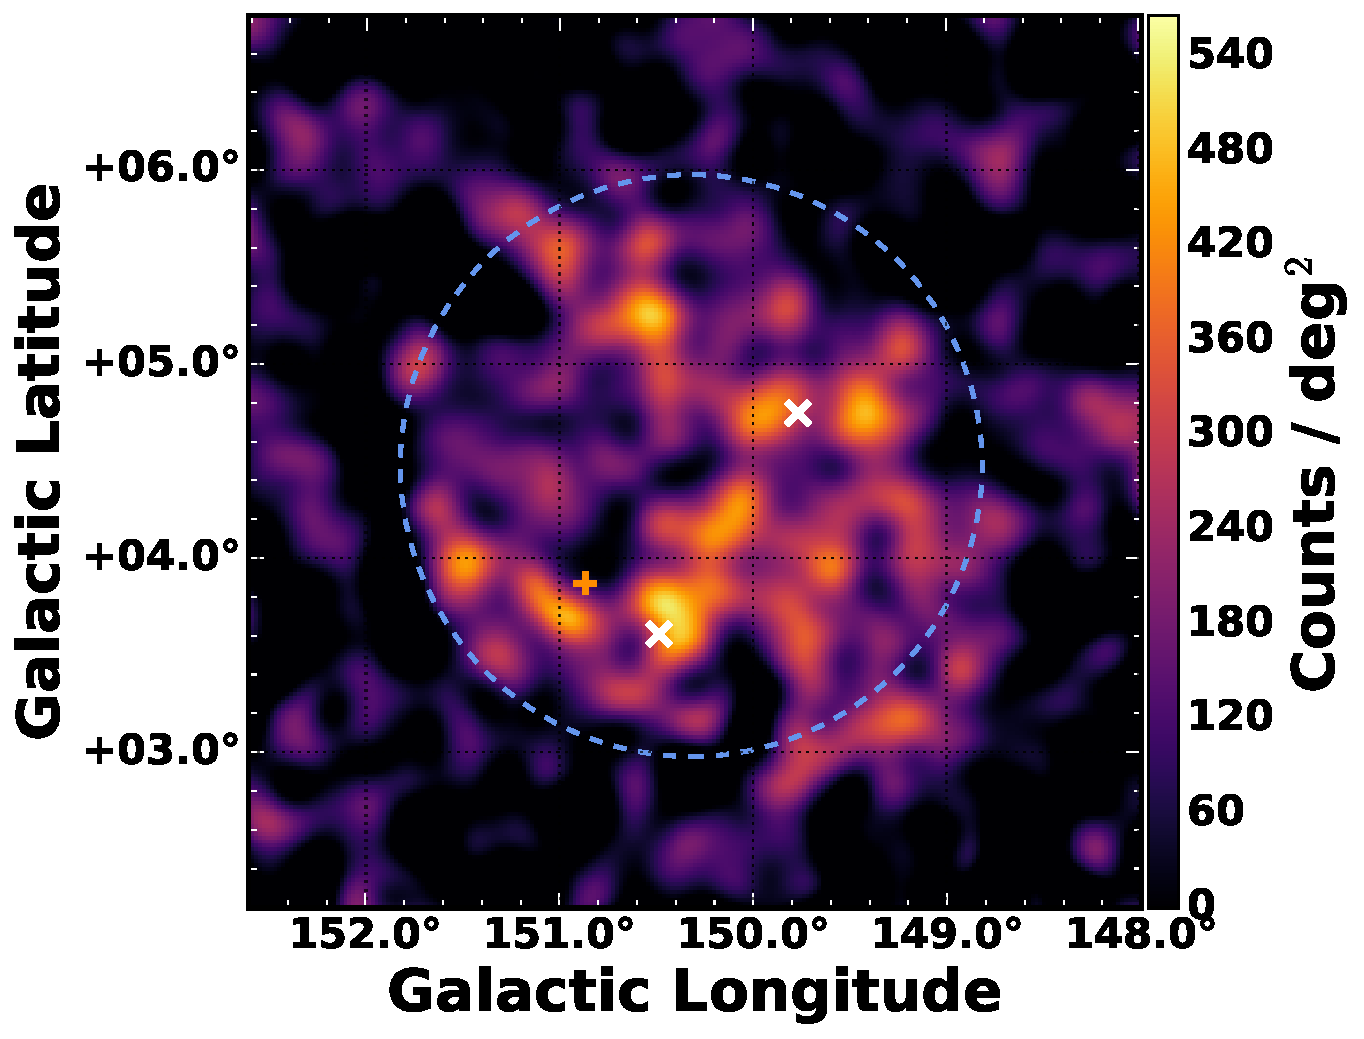
\includegraphics[width=1.\columnwidth]{Figures/G150/G150_1GeV_source_w3FGL_noLabs.pdf}
		\caption[Smoothed background subtracted residual counts map above 1 GeV for \Gone{}]{Smoothed background subtracted residual counts map above 1 GeV where 0.1$^\circ$x 0.1$^\circ$ pixels were smoothed with a Gaussian kernel of 0.1$^\circ$, centered on SNR \Gone. \psrLike{} and the diffuse backgrounds are included in the region model, 3FGL J0425.8+5600 and 3FGL J0423.5+5442 are not (but their locations are shown as white crosses). %Inset shows the size of the PSF above 1 GeV, demonstrating the \gam{} emission is extended well beyond the extent of the inset PSF
			\label{fig:1GeV_cmaps}}
	\end{centering}
\end{figure}

In our analysis, we removed 3FGL J0425.8+5600 and 3FGL J0423.5+544 from the RoI, but kept \psrLike{} in the model since preliminary analyses showed clear positive residual emission at the position of the source if it was removed from the RoI. Figure \ref{fig:1GeV_resTSmap} shows a residual TS map for the region around \Gone. This point source detection-significance map was created by placing a point source modeled with a power law of photon index $\Gamma$ = 2  at each pixel and gives the significance of detecting a point source at each location above the background. 

%put file name in {} to get it to compile with dots in the name!
%for png, have to use pdfchain
\begin{figure}[!h]
	\begin{centering}
		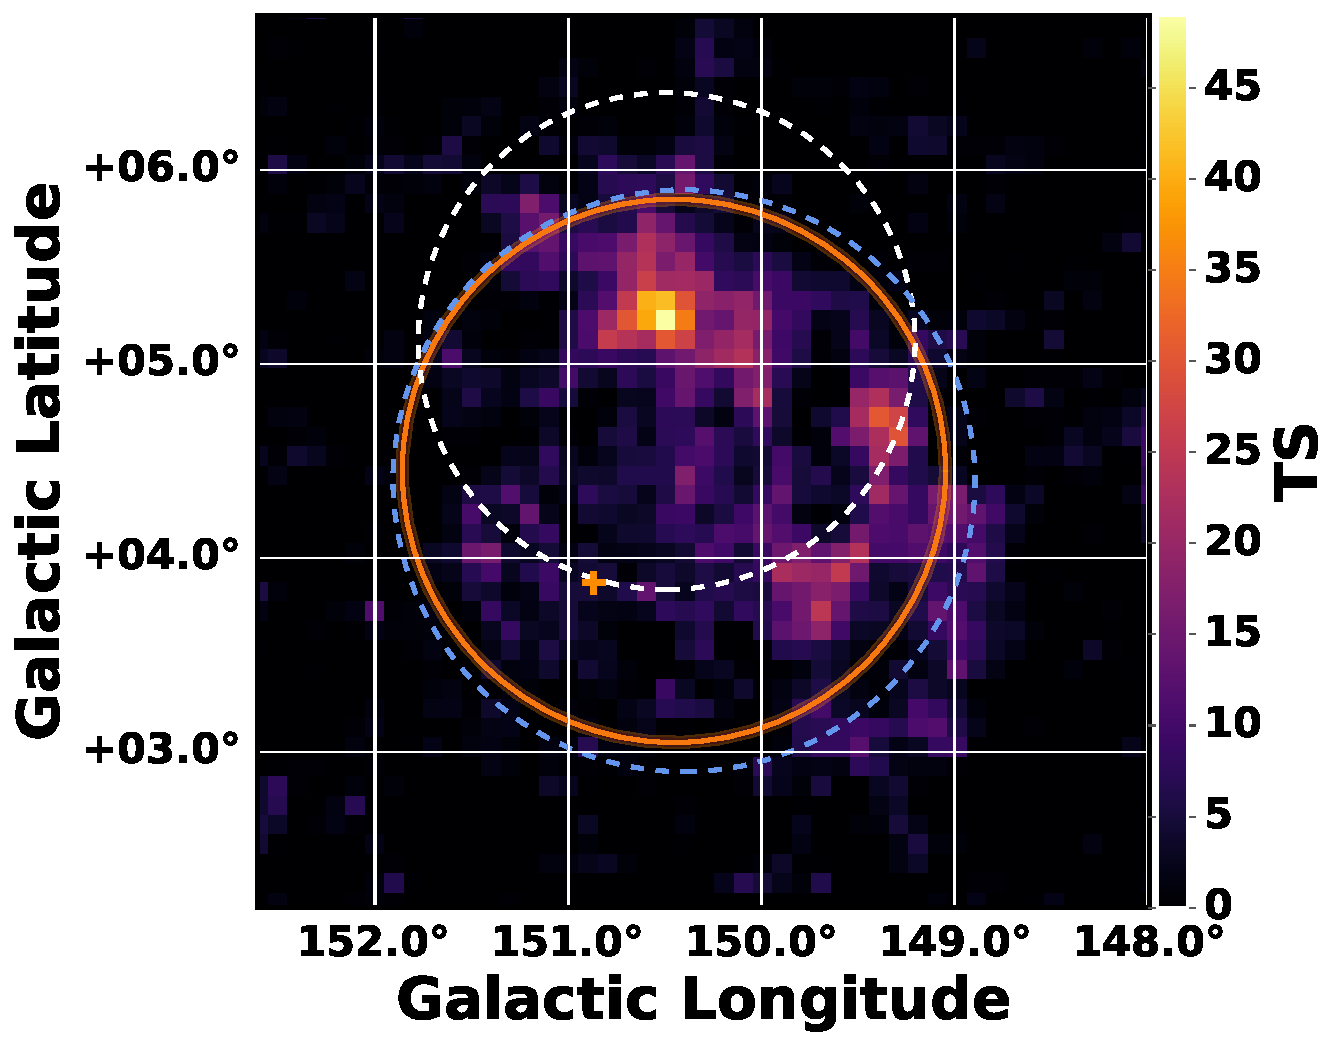
\includegraphics[width=0.85\columnwidth]{{Figures/G150/G150_1GeV_resTsmap_radio_2FHL_noLabs}.pdf}
		\includegraphics[width=0.85\columnwidth]{{Figures/G150/G150_1GeV_resTsmapNoG150_radio_2FHL_noLabs}.pdf}
		\caption[\Gone{} background subtracted residual TS map above 1 GeV]{Background subtracted residual TS map above 1 GeV with 0.1$^\circ$x 0.1$^\circ$ pixels, centered on SNR \Gone{}. The orange circle and translucent shading show the fit disk radius and 1$\sigma$ errors, respectively, for the extended source, the orange cross shows the position of \psrLike{} (included in the background model), blue dashed circle is the extent of the radio SNR, and white dashed circle depicts \ghard{}. Bottom map includes \Gone{} in the background model, top does not.
			\label{fig:1GeV_resTSmap}}
	\end{centering}
\end{figure}

We modeled the excess emission in the direction of \Gone{} with a uniform intensity, radially-symmetric disk, simultaneously fitting the spatial and spectral components of the model  via \ptlike{}. The extension of the disk was initialized with a seed radius of $\sigma$ = 0.1$^\circ$ and position centered on the radio position of \Gone{}. We define the significance of extension as in \cite{Lande12}; ${\rm TS_{ext} = 2~log(\mathcal{L}_{ext} / \mathcal{L}_{ps})}$, with $\mathcal{L}_{ext}$ being the likelihood of the model with the extended source and $\mathcal{L}_{ps}$ that of a point source located at the peak of emission interior to the extended source. For the disk model we found that  ${\rm TS_{ext} = 298}$, for the best fit radius, ${\rm \sigma = 1.40^\circ \pm 0.03^\circ}$, and position,  ${\rm R.A. = 55.46^\circ \pm 0.03^\circ }$, ${\rm DEC. = 66.91^\circ \pm 0.03^\circ }$, all in excellent agreement with the radio SNR size and centroid determined in \cite{Gao14}. Figure \ref{fig:radInt} shows radially integrated counts for the region as a function of angular radius squared. It's clear from this figure that there is significant excess of counts above the Galactic diffuse radiation in this region that is adequately modeled by a symmetric disk. We tried adding back in to our model the two removed 3FGL sources but both were insignificant when fit on top of the best fit disk. The bottom map in Figure \ref{fig:1GeV_resTSmap} is a residual TS map of the same region as the top map, but with the disk source included in the background model, demonstrating that the disk can account well for the emission in the region and justifying the exclusion of the two aforementioned 3FGL sources.

\begin{figure}[!ht]
	\begin{centering}
		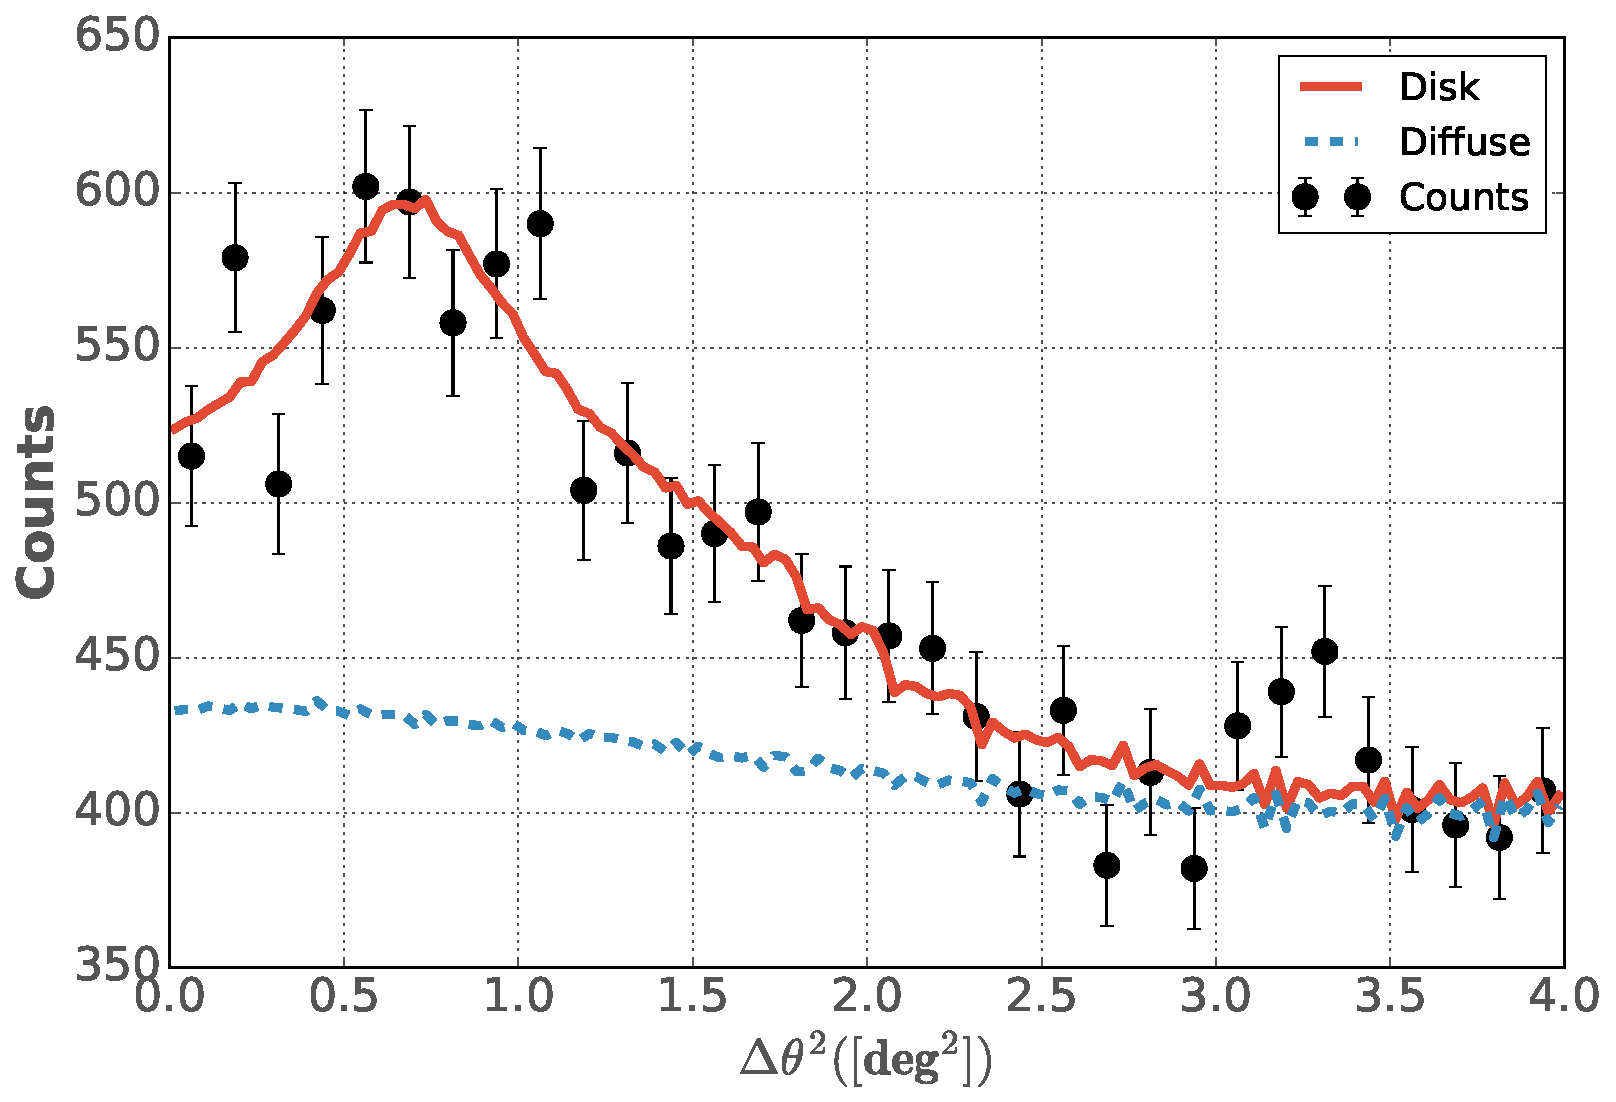
\includegraphics[width=\columnwidth]{{Figures/G150/G150_radInt_noPt}.pdf}
		\caption[G150 radially integrated counts map]{Radially integrated counts map centered on the GeV emission coincident with \Gone{}.  Red line shows the expected counts for a uniform intensity disk with radius,${\rm \sigma = 1.40^\circ}$, blue line is that of the Galactic diffuse background. 
			\label{fig:radInt}}
	\end{centering}
\end{figure}

The morphology of the radio emission is suggestive of an elliptical or ring morphology, so both of these spatial models were tested as well. For the ring model, the fit reduced to a disk with parameters matching those stated above. Using the elliptical model showed a weak improvement over the radially symmetric model at the 2.6$\sigma$ level (${\rm \Delta TS = 9}$ with two additional degrees of freedom), which we did not consider significant enough to say the GeV emission had an elliptical morphology (see Table \ref{tab:LATres}). For the remainder of this study, we only considered the disk spatial model.

\ghard{} is the extended source detected in the 2FHL catalog found to be overlapping the northern region of \Gone{} \cite{2FHL}. The source has a power law spectral index ${\rm \Gamma = 1.66 \pm 0.2}$, and disk radius ${\rm \sigma = 1.27^\circ \pm 0.04^\circ}$ (see Figure \ref{fig:1GeV_resTSmap}). When comparing the best fit extension of the 2FHL source with the result from this paper, factoring in the uncertainty in both extension and position, we see that the $>$ 50 GeV and $>$ 1 GeV results are not incompatible. It is likely that the paucity of events above 50 GeV is the cause of the smaller fit radius, as opposed to the difference arising from the effects of an energy dependent morphology. To explore the connection between the 2FHL and above 1 GeV emission, we tested a few other spatial hypotheses.

First, we  replaced the ${\rm \sigma = 1.40^{\circ}}$ disk with an another disk matching the spectral and spatial parameters of \ghard{} and calculated the likelihood with this new source's position and extension fixed. For this hypothesis, we find ${\rm TS_{ext} =  165}$, and  ${\rm TS = 226}$, demonstrating that the fixed disk matching the 2FHL source is clearly disfavored over the previously determined best fit disk at this energy. Our next test consisted of placing a second extended source on top of the best fit disk detected above 1 GeV. We added a source, initially matching the spatial and spectral parameters of \ghard{}, to our source model of the region (in addition to the ${\rm \sigma = 1.40^{\circ}}$ disk), and fit its spectrum and extension. Fitting a second extended source in this region serves two purposes: 1. it acts as a check on whether there was residual emission unaccounted for by the previously best-fit disk, and 2. it allows us to determine if the best fit disk can be split into two spectrally distinct, components. This fit resulted in the source wandering north (but still partially overlapping \Gone{}) and having an insignificant extension, ${\rm TS_{ext} =  4}$. Details on the spatial parameters are given in Table \ref{tab:LATres}.

\begin{deluxetable}{ccccccc}
\setlength{\tabcolsep}{0.04in}
\tablewidth{0pt}
\tabletypesize{\scriptsize}
\tcap{\Gone{} Extended Source Analysis Results\label{tab:LATres}}
\tablehead{
\colhead{Spatial Model} & 
\colhead{TS${\rm _{ext}}$} &
\colhead{TS\tablenotemark{a}} & 
\colhead{$\sigma$ [$^\circ$]} &
\colhead{R.A. [$^\circ$]} &
\colhead{DEC [$^\circ$]} & %\\
\colhead{Index}}
%\colhead{} & 
%\colhead{} & 
%\colhead{} &
%\colhead{} &
%\colhead{} &
%\colhead{}
\startdata
Disk             &    298  &     410 &  $1.40^\circ \pm 0.03^\circ$  & $55.46^\circ \pm 0.03^\circ$          & $66.91^\circ \pm 0.03^\circ$ & $1.82 \pm 0.04$  \\
Elliptical Disk  &    189.048 &   34 &  $1.78^\circ / 1.23^\circ \pm 0.02^\circ$  & $66.61^\circ \pm 0.04^\circ$ & $55.43^\circ \ pm 0.03^\circ$   & $1.86 \pm 0.04$ \\
2FHL (free)\tablenotemark{b}  &    260.317 &     17  &  $0.80^\circ \pm 0.04^\circ$  & $69.33^\circ \pm 0.06^\circ$      & $56.00^\circ \pm 0.06^\circ$ & $1.34 \pm 0.17$   \\
%2FHL (fixed) &    260.317 &     -3.277  &  63.87  & Puppis A      & snr    & 1.4\\
Disk \& 2FHL\tablenotemark{b}     & 4 &     17  &  $0.80^\circ \pm 0.04^\circ$  & $69.33^\circ \pm 0.06^\circ$      & $56.00^\circ \pm 0.06^\circ$ & $1.34 \pm 0.17$   \\

%\cutinhead{Thee Point Sources}
%\sidehead{Uniform Disk}
\enddata
\tablecomments{~ 2FHL (free) corresonds to the model where a disk matching \ghard{}, was included in the likelihood model and the spectral and spatial parameters we free to vary. For the 2FHL (fixed) model, \ghard{} was included with spatial parameters fixed. In the Disk \& 2FHL model, we included both the best-fit disk determined in $\S$\ref{sec:LATmorph}, fixed in position and size, and added a source resembling the \ghard{} with free spectral and spatial parameters. This model reports the fit values of \ghard{}
 }

\tablenotetext{a}{Calculated in \gtlike}
\tablenotetext{b}{Started with disk matching the spectral/spatial parameters of \ghard{}, then left them free to fit in the likelihood model.}
\end{deluxetable}




                


%\begin{figure}[!ht]
%   \begin{centering}
%       \includegraphics[width=\columnwidth]{{G150_extProf_1GeV}.png}
%       \includegraphics[width=\columnwidth]{{TSextVsEn_G150_1GeV_1TeV_sigma1_4}.png}
%       \caption{Not sure I want to include these, replot, get rid of titles, and make them look nicer if I do want to include. Top plot shows that the TS peaks at the best fit extension. Lower plot gives a sense of how significant the extension is (vs a point source) across the analyzed energy range. If I keep, add text in the section
%           \label{fig:extProf}}
%   \end{centering}
%\end{figure}
%%%%%%

\subsection{Spectral Analysis}\label{G150:LATspec}
After determining the best fit morphology with \ptlike{} for the GeV emission coincident with SNR \Gone{}, we used those results as a starting point for our \gtlike{} maximum-likelihood fit of the region to estimate the best spectral parameters for our model. The LAT data is well described by a power law from 1 GeV to 1 TeV with a photon index, ${\rm \Gamma = 1.82 \pm 0.04}$, and energy flux above 1 GeV of ${\rm (7.3 \pm 0.72)~ x 10^{-11}~ erg~cm^{-2}~ s^{-1}}$  and TS = 389 \jamie{pointlike results were index = 1.80 flux = ${\rm (7.17 \pm 0.73~ x 10^{-11})~ erg~cm^{-2}~ s^{-1}}$}. We tested the \gam{} spectrum of the extended disk for spectral curvature using a log-normal model (Log Parabola), and find no significant deviation from a power law (${\rm \Delta TS \sim 1}$). Figure \ref{fig:G150SED} shows the best-fit power law spectral energy distribution for the GeV source whose morphology was described in Section $\ref{G150:LATmorph}$. Spectral data points were obtained by dividing the energy range into 12 logarithmically spaced bins and modeling the source with a power law of fixed spectra index, ${\rm \Gamma = 2}$. We overplotted the SED of \psrLike{} to demonstrate how the spectra of the two sources are comparable in the lowest energy bin and would grow more confused at energies below 1 GeV.

%%%G150 pointlike SED: G150_1GeV_resTsmap_radio_noLabs.pdf
\begin{figure}[!ht]
	\begin{centering}
		\includegraphics[width=\columnwidth]{Figures/G150/{G150_J0426_SED}.pdf}
		\caption[Spectral energy distribution of \Gone{} and \psrLike{}]{Spectral energy distribution for the extended source coincident with SNR \Gone{} from 1 GeV to 1 TeV. Red line corresponds to the best-fit power law model. Points are shown with with statistical error bars. Grey dashed line is the SED of \psrLike{}, modeled with an exponential cut-off power law.
			\label{fig:G150SED}}
	\end{centering}
\end{figure}

%pointlike SED G150.3+4.5_3FGLJ0426.7+5437_SED.png
%\begin{figure}[!ht]
%   \begin{centering}
%       \includegraphics[width=\columnwidth]{Figures/{3FGL_J0426.7+5437_gtlike_defaultBkgRefit_SED}.pdf}
%       \caption{Spectral energy distribution of \psrLike{}. \jamie{Get rid of this!. Replot the G150 SED with this J0425 overlayed}
%           \label{fig:J0426SED}}
%   \end{centering}
%\end{figure}


%%%%%%%%%%%%%%%%%%%%%%%%%%%%%%%%%%%%%%%%%%%%%%%%%%%%%%%%%%%%%%%%
%
%         Multiwavelength  Observations and  Analysis 
%
%%%%%%%%%%%%%%%%%%%%%%%%%%%%%%%%%%%%%%%%%%%%%%%%%%%%%%%%%%%%%%%%

\section{Multiwavelength  Observations and  Analysis }\label{G150:Multiwave}
\subsection{HI}\label{G150:HI}
\jamie{Jack is working on this}
%\subsection{CO?}\label{G150:CO}
%\jamie{Jack's looking into Planck data for HI and CO}
\subsection{X-ray}\label{G150:Xray}
\jamie{Dan is working on this.}

%\jamie{No diffuse nonthermal X-ray emission observed by ROSAT. No point sources near the center? Should a  pulsar even  be near the center?}

%\jamie{Place a limit on ambient density with an upper limit on thermal X-ray emission.  upper limit on potential pulsar spin-down power, then see what fraction of that power the lum of J0426 would be, assuming it's at the distance of G150 to see if that's reasonable for it being the putative pulsar?}

%\jamie{When I have the xray flux, Can I say what edot of the psr would be if I know the LAT flux and xray flux? here's the flux detected from G150... assuming the derived distance, here's the luminosity...If it's a PWN does this luminosity suggest a spindown power?...or at least what fraction of some reasonable spin down power is this lum?...If we have an upper limit on the x-ray flux, does the ration of x-ray to gamma suggest a spin down power?...which paper I was looking at today mentioned the connection between xray lum and psr spin down power? W41 parer does something, but I thought there was another? Look at Dan's W41 too, and MSH 11-61A something like Mattana et al. 2009 correlation between  $\mathrm{flux_x / flux_g \propto}$   Edot?} 
%%%%%%%%%%%%%%%%%%%%%%%%%%%%%%%%%%%%%%%%%%%%%%%%%%%%%%%%%%%%%%%%
%
%         Discussion and Results
%
%%%%%%%%%%%%%%%%%%%%%%%%%%%%%%%%%%%%%%%%%%%%%%%%%%%%%%%%%%%%%%%%
\section{Discussion and Results}\label{G150:Discuss}
\subsection{SNR or PWN?}\label{G150:PWNvsSNR}

The follow-up observations of the \gam{} emission in the direction of \Gone{}, presented here, of the source detected above 50 GeV in 2FHL have led to the detection of an extended \gam{} source whose centroid and radius match extremely well with those of the radio detected SNR. The broad size of the extended source and correlation with the radio shell leave few plausible scenarios for the nature of the GeV emission. Namely, the GeV emission can arise from the wind nebula of the putative pulsar of \Gone{} or the GeV emission corresponds to \gam{}s produced in the SNR. We argue here that the SNR is favored over a pulsar wind nebulae (PWN) as the generator of the observed \gam{}s.

The first problem with the PWN hypothesis is that there is no pulsar candidate detected near the centroid of the SNR to power a PWN. While 3FGL J0425.8+5600 is the closest \gam{} source to the center of the remnant, it does not have a pulsar-esque spectrum, it lies about ${\rm 0.25^\circ }$ away, and we showed in Chapter \ref{G150:LATmorph} that with the best-fit disk hypothesis, neither 3FGL J0425.8+5600 nor 3FGL J0423.5+5442 are significant in the likelihood model of the region. \psrLike{}, with a spectrum reminiscent of a pulsar,  may actually be one, but as discussed previously, \cite{Barr13} detect no pulsations from the source \jamie{something to say about SWIFT nondetection?}). Furthermore, the source is $0.84^\circ$ away from the centroid of \Gone{}. Typical pulsar ballistic velocities range from ${\rm V_{PSR} \sim 400-500~km~s^{-1}}$, with extreme velocities exceeding ${\rm 1000~km~s^{-1}}$ \citep{Gaensler06}. If \psrLike{} was the compact remnant of the progenitor star that birthed \Gone{}, it would have to be traveling with a velocity, ${\rm V_{PSR} = 1125~km~s^{-1}}$ (assuming an age of 5 kyr, which we derive in the following section, Chapter \ref{G150:SNRevo}), and would make it one of the fastest known pulsars \citep{Chatterjee05}. While possible, this scenario is unlikely without further evidence to support such a high velocity. \jamie{Fastest pulsar (till 2011 at least) 1100 km/s, more recent ref?}]

Another argument disfavoring the PWN scenario is that, despite the hard \gam{} spectral index extending to TeV energies, ROSAT X-ray observations detect no significant emission suggestive of a PWN in the direction of \Gone{} (see Chapter \ref{G150:Xray}). Typical PWNe spectral indices range from about $-0.3 \lesssim \alpha  \lesssim  0$ \citep{Gaensler06}. The radio spectral index  as determined in \cite{Gao14}  ($\alpha = 0.4 \pm 0.17$ for part of the eastern shell, $\alpha = 0.69 \pm 0.24$ for a region in western shell) suggests that the radio object is likely not a PWN.

Many of the arguments disfavoring the PWN hypothesis in fact bolster that of SNR. First and foremost in favor of an SNR origin for the \gam{} emission is the excellent agreement between the GeV best-fit disk radius and centroid with that of the radio shell.  The radio shell-like appearance, non-thermal radio spectrum, and strands of red optical filamentary structures led both \cite{Gao14} and \cite{Gerbrandt14} to regard the radio source an SNR as opposed to a PWN.  The radio spectral index, while not quite in line with typical PWN spectra, is actually  common of SNRs.

While the above factors lend credence to an SNR origin for the GeV \gam{}s the PWN  scenario can not be ruled out due to the lack of an associated pulsar. Regardless, for the remainder of this study, we assumed the observed\gam{}s were produced in the shock front of SNR \Gone{}

\subsection{\Gone{} in an \snr{} Context }\label{G150:SNRevo}

Having associated the \gam{} emission with \Gone{}, next, we assessed the evolutionary state of the remnant to place it in context within the current population of LAT SNRs. Using the most viable HI kinematic distance, ${\rm d  \approx 0.38~kpc}$ derived in Chapter \ref{G150:HI}, we showed that the projected radius of \Gone{} is ${\rm R \approx 9.4~pc}$. Employing a standard Sedov-Taylor solution for the expansion of a blast wave, we estimated the age of \Gone{}. In the Sedov phase, the radius of the shock front is given by,

%\begin{equation}
%/R_{12.5} = \bigg{(}\frac{E_{51}}{n_0} \bigg{)}^{1/5} t_4^{2/5}
%\end{equation}

\begin{equation} \label{eq:ST}
	R_{ST} = 0.314 \bigg{(}\frac{E_{51}}{n_0} \bigg{)}^{1/5} t_{{\rm yr}}^{2/5} {\rm  pc}
\end{equation}

\jamie{None of this is taking into account the low density upper limit. give Age for a few n's}
Where ${\rm E_{51}}$ is the kinetic energy output of the  supernova in units of ${\rm 10^{51}~erg}$, and ${\rm n_0}$ the ambient density the shock is expanding into in units of ${\rm cm^{-3}}$. Assuming standard values of 1 for ${\rm E_{51}}$ and ${\rm n_0}$ we solved equation \ref{eq:ST} for ${\rm t_{yr}}$ (the current age of the remnant in years) and used the value of R derived for \Gone{} to estimate the age of the SNR as ${\rm t \approx 4.9~kyr}$.%\jamie{Figures \ref{fig:LATseds} and \ref{fig:LvsD2} demonstrate how the properties of \Gone{} compare to those of other LAT SNRs of various age.}

Figure \ref{fig:LATseds} shows the SED of \Gone{} overlaid on the spectra of a selection of other LAT observed SNRs with ages ranging from ${\rm\sim  10^3 - 10^4 yr}$. \Gone{} exhibits a hard spectrum extending to TeV energies with no spectral break (breaks are commonly seen in LAT SNRs interacting with nearby molecular material \citep{Hewitt15}) and appears spectrally similar to the younger SNRs like RX J1713.7-3946 and RX J0852.0-4622. In figure \ref{fig:LvsD2}, we plotted the luminosity of several LAT SNRs against their squared diameters (a proxy for age, as evident from equation \ref{eq:ST}). \jamie{should be using SNR cat fig 18?. need to reword things if I'm just taking their figure and putting my points on}. Similarly, with it's low luminosity \jamie{give L here. If I use the W41 LvsD2 plot, 100MeV-100 GeV, if SNR cat, 1-100 GeV}, \Gone{} appears to correlate well with the younger sect of LAT SNRs.
Our age estimate alone does not unambiguously determine the evolutionary state of \Gone{}. However, when combined with the results of Figures \ref{fig:LATseds} and \ref{fig:LvsD2} comparing \Gone{} to the population of other LAT SNRs, it indicates that \Gone{} is more compatible with a dynamically unevolved, non-interacting (with the surrounding interstellar medium) stage of expansion.

%\jamie{The age of an SNR in the Sedov phase is not always an unambiguous determinant of the remnants evolutionary phase. An age of ${\rm \sim 5~kyr}$, falls into this grey area straddling the so-called young (${\rm few \times 10^3 yr}$) middle-aged (${\rm  few \times 10^4 yr}$)}  In Figure $\S$\ref{fig:LATseds}, we show the SED of \Gone{} overlaid on a representative sample of SEDs of other LAT observed SNRs with ages ranging from ${\rm\sim  10^3 - 10^4 yr}}$. 

\begin{figure}[!ht]
	\begin{centering}
		\includegraphics[width=\columnwidth]{Figures/G150/{G150_SEDall_overlay}.pdf}
		\caption[SEDs for several LAT observed SNRs]{SEDs for several LAT observed SNRs with ages spanning ${\rm\sim  10^3 - 10^4 yr}$. SNRs less than 10 kyr are plotted as squares, older plotted as circles.  The GeV spectrum of  \Gone{} is shown as stars.  \jamie{I need refs for each}
			\label{fig:LATseds}}
	\end{centering}
\end{figure}

\begin{figure}[!ht]
	\begin{centering}
		\includegraphics[width=\columnwidth]{Figures/G150/{G150_LvsD2_60pc}.pdf}
		\caption[Luminosity versus squared diameter for several LAT SNRs.]{Luminosity of several LAT SNRs plotted against their \jamie{radio? GeV?} diameter squared. \jamie{taken from W41 paper, overplotted G150} \jamie{Should I actually remake this myself or is it ok to just use the one from the other paper with my points on it? Add more text when I settle on a plot.}
			\label{fig:LvsD2}}
	\end{centering}
\end{figure}

\subsection{Nonthermal Modeling}\label{G150:naima}


SNR shock fronts are known accelerators of cosmic rays to very high energies. There are potentially multiple radiation mechanisms operating at the shock that produce GeV \gam{}s. Accelerated electrons can give rise to inverse Compton (IC) emission via upscattering of ambient cosmic microwave background (CMB), stellar, and IR photon fields, as well as non-thermal bremsstrahlung radiation. Energetic protons can collide with ambient protons in the surrounding, producing neutral pions which decay into \gam{} photons. 

To infer the properties of the underlying relativistic particle populations in the SNR environment, it is vital to understand the origin of the observed \gam{} emission detected from  \Gone{}. To do so, we employ the \nai{} Python package. \nai{} is an open-source code base that computes the non-thermal radiation from a relativistic particle population \citep{Zabalza15}. It utilizes known parameterizations and analytic approximations to the various non-thermal processes (i.e., synchrotron, IC, bremsstrahlung, and pion decay emission), which results in the calculations being computationally inexpensive. \nai{} also makes use of \emc{}, a Markov chain Monte Carlo (MCMC) ensemble sampler for Bayesian parameter estimation \citep{Foreman13}. The sampler is used to find the best-fit parameters of the radiative models to the observed photon SED for a given particle distribution function. 

To determine the best fit parameters, \nai{} calls \emc{} to sample the log-likelihood function (i.e., the likelihood of the observed data given the assumed spectrum) of the radiative model.\jamie{should I include what the likelihood function looks like here?} The radiative models require as input a particle distribution function to model the present-age electron or proton spectrum. We used a one-zone, homogeneous particle distribution model (which \nai{} inherently assumes) and scaled the likelihood function by a uniform prior probability distribution. For this work, we model the separate proton and electron and spectra as power laws with an exponential cut off,

\begin{equation}\label{eq:ecpl}
	{\rm \frac{dN}{dE}_{(e,p)} = A_{(e,p)} (E / E_0) ^{-s} \exp {\bigg ( }\frac{- E}{ E_{cutoff~(e,p)}}{\bigg)}}
\end{equation}

where E is the particle energy, ${\rm E_0}$ the reference energy, s the spectral index, and ${\rm E_{cutoff}}$ the cutoff energy. The electron distribution's normalization is related to the proton normalization through the electron-to-proton ratio scaling factor, $A_e = K_{ep} A_p$. We also assumed that the electron and proton distributions have the same spectral shape.

For our radiation models, we assumed a gas density, ${\rm n_0 = 1~cm^{-3}}$ for proton-proton \jamie{and bremss when I get it working} interactions For IC emission, we include CMB  (
Talk about free/ fixed params of the model, reference the table, and figure to show best fit, discuss results and what the fits imply regarding lep/had dom and energy in e- p.

\jamie{Used radio SED from \citep{Gerbrandt14}}

\begin{deluxetable}{cccccc}
\setlength{\tabcolsep}{0.04in}
\tablewidth{0pt}
\tabletypesize{\scriptsize}
\tcap{Naima Model Best Fit Parameters\label{tab:naima}}
\tablehead{
\colhead{s} & 
\colhead{${\rm K_{ep}}$} & 
\colhead{${\rm A_p}$ } &
\colhead{B\tablenotemark{a}} & 
\colhead{${\rm E_{cutoff(e)}}$} &
\colhead{${\rm E_{cutoff (p)}}$}} %\\
%\colhead{} & 
%\colhead{} & 
%\colhead{${\rm 10^48}~TeV^{-1}$  } &
%\colhead{} &
%\colhead{} &
%\colhead{}
\startdata
\sidehead{\underline{Fixed ${\rm K_{ep}} = 0.01$}}
1.5 $\pm$ 0.2     &    0.01 &     -32.850 &  49.80  & LMC   & 2 \\ 

\sidehead{\underline{Fixed ${\rm K_{ep}} = 0.1$}}
1.5 $\pm$ 0.2    &    0.1 &     -3.277  &  63.87  & Puppis A    & 2    \\

\sidehead{\underline{Fixed ${\rm K_{ep}} =1$}}
1.5 $\pm$ 0.2    &    1 &     -3.277  &  63.87  & Puppis A      & 2 \\

\sidehead{\underline{Fixed s}}
2 $\pm$ 0.2    &    1 &     -3.277  &  63.87  & Puppis A      & 2 \\
%\sidehead{Uniform Disk}

\enddata
\tablecomments{~ \jamie{add better caption} Results from naima model?  Right now the free params are index, kep, eleccut, protcut, B. Fixed are nh, all the IC photon field values distance (this is just for determining flux) \jamie{Correct values aren't in yet}\jamie{}add units to params}

\tablenotetext{a}{Calculated in \gtlike}
\end{deluxetable}


\jamie{estimates min of negative loglike through sampling}  

\jamie{Say something about what the radio index is and the connection to the gev index}

%\jamie{use ratio of \gam{} to radio flux to set kep, assuming it's hadron dom? I can't remember what paper I saw  this in.}

\jamie{Discuss implications of the naima fits. Do they show preference for lep/had? suggest something about total energy content in particles?}



\begin{figure}[!ht]
	\begin{centering}
		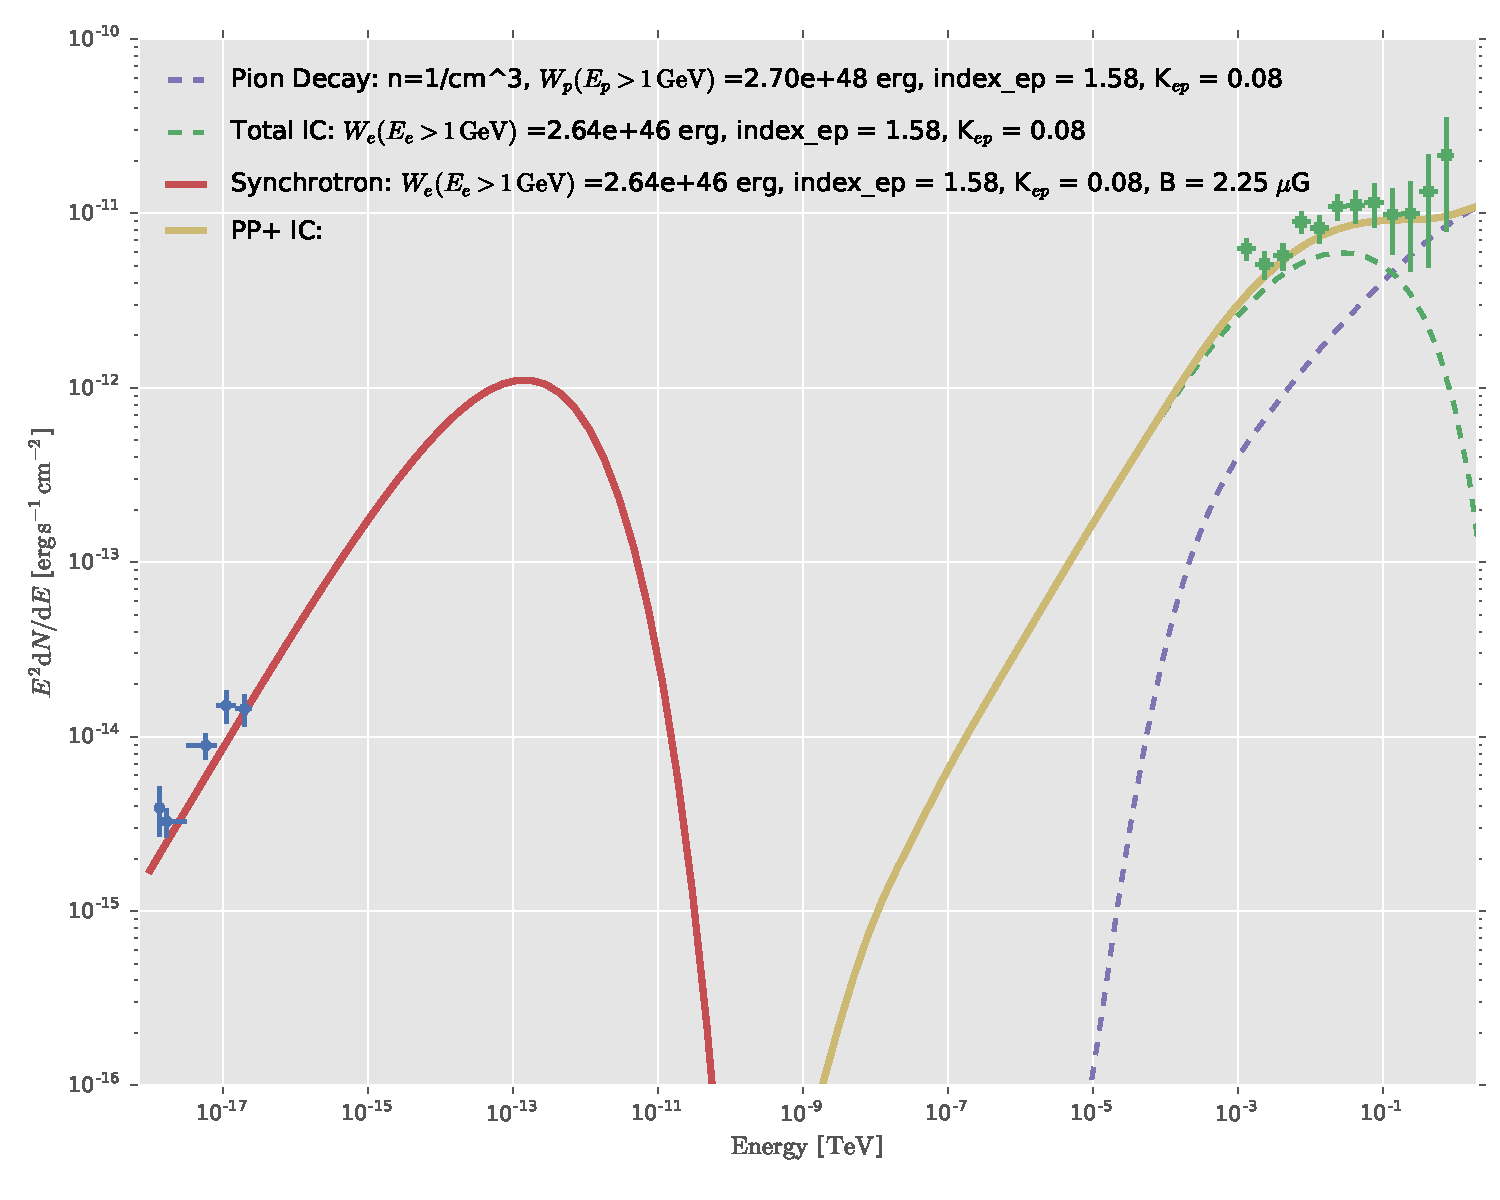
\includegraphics[width=\columnwidth]{Figures/G150/G150_ICsync_PP_SED.pdf}
		\caption[Non-theraml emission model for \Gone{}]{ \Gone. Naima SED \jamie{bigger font, get rid of text for each line, better colors}
			\label{fig:naimaSED}}
	\end{centering}
\end{figure}

\jamie{Another section here? can I just put a paragraph about what future observations will  elucidate on in the conclusions?}

\jamie{looks like young SNRs, but no x-ray and lower luminosity than most other LAT SNRs. It's possibly just that ROSAT is no sensitive enough.}

\jamie{Deeper x-ray observations to search for the compact stellar remnant. ROSAT all-sky not that sensitive, dedicated X-ray to search for thermal/nonthermal components}

\jamie{What can be done in TeV? The difficulty pointed TeV observations are that it might be difficulty for them to detect such broadly extended emission (why? I know they'd have to tile their observations, but there's something inherently difficulty for them about observing large extended sources. Is it just that the emission is spread out so it might be faint and below the detection threshold?). What about HAWC? Why does it not detect the emission that Fermi clearly shows extending to VHE energies? Is it not as sensitive at this energy for some reason? HAWC energy range extends to 100 GeV.}


%%%%%%%%%%%%%%%%%%%%%%%%%%%%%%%%%%%%%%%%%%%%%%%%%%%%%%%%%%%%%%%%
%
%         Conclusion
%
%%%%%%%%%%%%%%%%%%%%%%%%%%%%%%%%%%%%%%%%%%%%%%%%%%%%%%%%%%%%%%%%
\section{Conclusions}\label{G150:Conc}
We analyzed 7 years of \FermiLat{} data in the direction of SNR \Gone{}, lowering the energy threshold from that previously reported in the 2FHL catalog, and report detection of significantly extended \gam{} emission coincident with the entirety of the radio remnant's shell. We find the emission from 1 GeV to 1 TeV to be well described by a power law of spectral index ${\Gamma = \rm 1.82 \pm 0.04}$, with  morphology consistent with a uniform disk with best-fit radius, {\rm $\sigma = 1.40^{\circ} \pm 0.03^{\circ}$}.  Based on radio and  \gam{} properties of emission in the direction of \Gone{}, within the context of the current LAT SNR population, we argued that the GeV emission likely originates in the shock of \Gone{}, and disfavor a PWN origin. To estimate the distance to the SNR, we obtained  an HI spectrum toward \Gone{} from the Leiden/Argentine/Bonn survey of Galactic HI. Calculating distances from the derived HI velocity peaks, we showed that the most reasonable distance estimate places \Gone{} at a distance of ${\rm d = 0.4~kpc}$, making it one of the closest known SNRs detected by the LAT. Using this distance and a standard Sedov-Taylor SNR evolution model, we estimate the age of the \Gone{} to be ${\rm t \sim 5~kyr}$. Say something about X-ray once I know itTo assess the underlying particle population acting in \Gone{} we use the \nai{} Python package to fit the observed radio and \gam{} SED to non-thermal electron and proton radiation models. We find that blah, which suggests more blah. Something about how G150  fits in with other LAT detected SNRs based on age, spectrum luminosity, spectral modeling. End with what  further observations can get us.

\jamie{thanks?}

\section{Scratch}

${\rm L_{\gamma} = 1.3 \times 10^{33}~erg~s^{-1}}$ from 1 GeV to 1 TeV for best d and flux above


energy flux from 100 MeV to 100 GeV: ${\rm 4.84 \times 10^{-11}~erg~cm^{-2}~s^{-1}} $

${\rm L_{\gamma} = 8.6 \times 10^{32}~erg~s^{-1}}$ from 100 MeV to 100 GeV for best d and flux in same range

energy flux from 1 GeV to 100 GeV: ${\rm 3.83 \times 10^{-11}~erg~cm^{-2}~s^{-1}} $

${\rm L_{\gamma} = 6.8 \times 10^{32}~erg~s^{-1}}$ from 1 geV to 100 GeV for best d and flux in same range

For diamMax = 60pc, dmax = 1.22kpc, and Lmax (100mev-100GeV) = 8.7e+33

\jamie{One potential scenario is that the \gam{}s in this region are produced by a pulsar wind nebula (PWN) generated by the putative pulsar of SNR \Gone{}.} 

\jamie{for synchrotron $\alpha = (1-s)/2$, where $\alpha$ is the radio spectral index, and s the electron distribution power law index. Same for IC below break?}

\jamie{SNR cat figure 8 suggests there are only 4(ish) SNRs with an index less than 2}

\jamie{eastern shell (Jack called this overall) radio index $\alpha = 0.4 \pm 0.17$  \cite{Gao14}, but $\alpha = 0.69 \pm 0.24$ for the western}

\jamie{For energies below the high energy break, For pion and bremss $\Gamma = 2\alpha + 1$ (says SNR cat) For IC, $\Gamma = \alpha + 1 $ ) for positive $\alpha$}

\jamie{From \cite{Gaensler06} Typical indices for PWNe are $\sim -0.3 \lesssim \alpha  \lesssim  0$ in the radio band, and ($\Gamma \approx 2$) in the X-ray band. So $\alpha$ is not inconsistent, but at the boundary.}

\jamie{For puppis A paper, why did they use particle index = gam photon index?}

\jamie{cr abundances at earth kep = 0.01  (Hillas 2005). I think in the puppis A paper the use 0.02?}

\jamie{Sooo, my index is consistent with either?}

\jamie{how off can dist be? SNR catalog says 8 SNRs are withing 1.5 kpc and have some kind of classification in the catalog. These are (closest first) Vela, cygnus loop , Vela Jr, RX J1713, G073, S147, IC443, Monoceros loop. if 0.4 kpc is correct for G150, it's the second closest LAT detected SNR. Even at 1.5 kpc it would be within top 10}